\documentclass{article} 
\usepackage[margin=1in]{geometry}
\usepackage{adjustbox}
\usepackage{amsthm}
\usepackage{amssymb}
\usepackage{../../../18/misc/pset_environments}

\usepackage[hidelinks]{hyperref}
\hypersetup{
  colorlinks,
  citecolor=blue,
  linkcolor=blue!30!orange,
  urlcolor=blue}

\def\constcolor{\color{green!60!black}}
\def\lincolor{\color{orange}}
\def\expcolor{\color{red}}

\def\partspace{\hspace{7pt}}

\usepackage[backend=biber, maxbibnames=9, maxcitenames=9,style=alphabetic, sorting=ynt]{biblatex}
\addbibresource{references.bib}
\usepackage{microtype}

\begin{document}

\providetoggle{inputted}
\iftoggle{inputted}{
   \section{Draft}}{
\title{Grid-unfolding orthogonal polyhedra}
\author{Natalie Stewart}
\date{}
\maketitle
}

\abstract{
  Recent results are summarized in the open problem of grid-unfolding orthogonal polyhedra.
}

\begin{figure}
  \begin{center}
    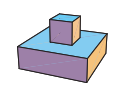
\includegraphics[width=.3\textwidth]{./figs/genus_0_orthogonal_polyhedron.png}
    \hspace{.1\textwidth}
    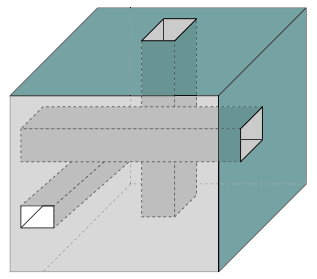
\includegraphics[width=.2\textwidth]{./figs/genus_3_orthogonal_polyhedron.png}
  \end{center}
  \caption{Two examples of orthogonal polyhedron.
  Neither posses an edge unfolding, and the right does not possess an orientation such that there exists a rim enclosing a face.
  The left figure is due to \cite[Fig. 22.4]{Demaine_textbook} and the right is due to \cite[Fig. 7.]{Damian_Demaine}.}\label{Orthogonal polyhedron figure}
\end{figure}

\section{Introduction}

In applications, it's often the case that one desires to manufacture a closed surface by cutting a 2-dimensional figure out of a flat plane and bending it into shape, fusing edges at the end.
The process of deciding a plan to do so--that is, choosing on the surface where the fused boundary will be, cutting, and unfolding to a figure of the plane--is of interest; see \cite{Kim,Wang}.

In computational geometry, the mathematical formulation of this problem centers around unfolding; how can a sufficiently nice surface be \emph{cut} and \emph{unfolded} into a sufficiently nice figure in the plane?
More specifically, given a surface bounding a polyhedron, how may we embed a graph into the polyhedron and isometrically map the complement of the graph onto a simple polygon?\footnote{The distance between two points in such a complement can be considered the infimum of the lengths (measured the usual way in $\mathbb{R}^3$) of all piecewise-linear paths lying on the complement of the graph with endpoints given by the two points.} 

We will often abuse language by referring to \emph{a polyhedron} when we mean its surface.
Without any restrictions on the graph used to cut the polyhedron, such an unfolding is called a \emph{general unfolding}.
Though convex polyhedra attain general unfoldings, it is currently unknown whether there exist general unfoldings of all nonconvex polyhedra \cite{Demaine_textbook}, so in order to find results we need to narrow the scope.

\begin{definition}
  An \emph{orthogonal polyhedron} is a polyhedron whose faces meet at right angles, and whose faces are each perpendicular to either the $x$, $y$, or $z$ axis.
\end{definition}
We'll henceforth work solely with orthogonal polyhedra.
These loosely appear to be made up of boxes nicely pasted together, with box-shaped dents or holes.
Some examples appear in Figure \ref{Orthogonal polyhedron figure}.


Another way to narrow the scope is to restrict the class of cuts which we can make;
motivated by manufacturing, one can restrict to \emph{edge unfoldings}, where the cuts may only be made along the edges of the polyhedron.
Then, there exist orthogonal polyhedra without edge unfoldings. 
Two such examples appears in Figure \ref{Orthogonal polyhedron figure}; 
in \cite{Demaine_textbook} it is shown that the graph involved in an unfolding must span the 1-skeleton of the polyhedron, so such a graph will not be connected.
However, this implies that the boundary of the polygon it folds to will not be connected, contradicting simplicity of the polygon.
In fact, it was proven in \cite{Abel_Demaine} that it is strongly NP-complete to decide whether an orthogonal polyhedron possesses edge unfoldings.


The middle ground most often struck in the case of orthogonal polyhedra is called \emph{grid unfolding.}
We replace an orthogonal polyhedron $P$ with another $P'$ formed by adding edges to $P$ formed by intersecting $P$ with planes parallel to the coordinate planes at each vertex, then replace $P'$ with some $P''$ which replaces each face of $P'$ with a $k \times k'$ grid of faces.
We refer to an edge unfolding of $P''$ as a \emph{grid unfolding of $P$ with $k \times k'$ refinement}, which we may picture as cutting along a grid on $P$ with ``resolution'' dictated by $k,k'$.

\begin{figure}
  \begin{center}
    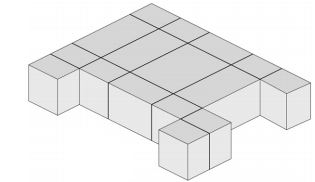
\includegraphics[width=.3\textwidth]{./figs/grid.png}
    \hspace{.1\textwidth}
    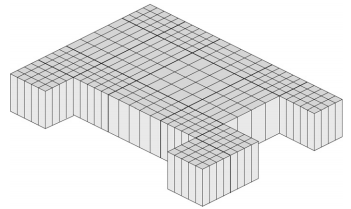
\includegraphics[width=.3\textwidth]{./figs/refined_grid.png}\\
  \end{center}
  \caption{On the left is an unrefined grid, and on the right is a grid with $4 \times 5$ refinement.
    This figure is due to \cite[Fig. 4]{Damian_Flatland_Orourke_Manhattan}.}
    \label{Grid refinement figure}
\end{figure}
\begin{figure}
    \adjustbox{max width=\textwidth}{
    \begin{tabular}{|c | c | c| c|}
            \hline
            Class & Refinement & Reference & Legend\\
            \hline
            \hline
            Orthogonal polyhedra & Open  & \cite{Damian_Flatland_Orourke} & (OP)\\ 
            Genus $g \leq 2$ orthogonal polyhedra & $O(n) \times O(n)$ & \cite{Chang_Yen,Damian_Demaine} & (OP$\leq$2))\\
            \hline
            Genus $g$ one-layer polyhedra & $2 \times 1$ on only $2(g-1)$ faces & \cite{Chang_Yen} & (OLOP)\\
            \hline
            Well-separated orthographs & $2 \times 1$ & \cite{Ho_Chang_Yen} & (WSOG)\\
            Orthotrees & $4 \times 4$ & \cite{Damian_Flatland,Damian_Flatland_Better} & (OTR)\\
            Orthotubes & $1 \times 1$ & \cite{Biedl_Demaine} & (OTU)\\
            Orthostacks & $2 \times 1$ & \cite{Biedl_Demaine} & (OST)\\
            Manhattan towers & $5 \times 4$ & \cite{Damian_Flatland_Orourke_Manhattan} & (MT)\\
            \hline
            Regular orthogonal polyhedra w/ $x-$ and $z-$holes & $2 \times 1$ & \cite{Ho_Chang_Yen} & (ROP$xz$)\\
            \hline
          \end{tabular}}
  \caption{A list of classes of orthogonal polyhedra where results are known.
    The legend column corresponds with Figure \ref{Results tree figure}.}\label{Results list figure}
\end{figure}
This motivates an open problem:
\emph{what are the smallest $k,k'$ such that every orthogonal polyhedron possesses a grid unfolding with $k \times k'$ refinement?}
In attempting to answer this, $k$ and $k'$ are often allowed to depend on the size $n$ of the data necessary to specify the polyhedron.
We are not aware of any answer or upper bound to this question in the general case;
instead, known results further restrict the orthogonal polyhedron into special cases.

Known results can be roughly separated into two types:
there are some fairly restrictive classes of orthogonal polyhedra which are known to be unfoldable with constant refinement, and there are some results which establish unfoldability with non-constant refinement for orthogonal polyhedra of low genus.
These results are summarized in Figure \ref{Results list figure}, and the relationships between the different classes are shown in Figure \ref{Results tree figure}.
\begin{figure}
  \begin{center}  
   \adjustbox{max width=.8\textwidth}{   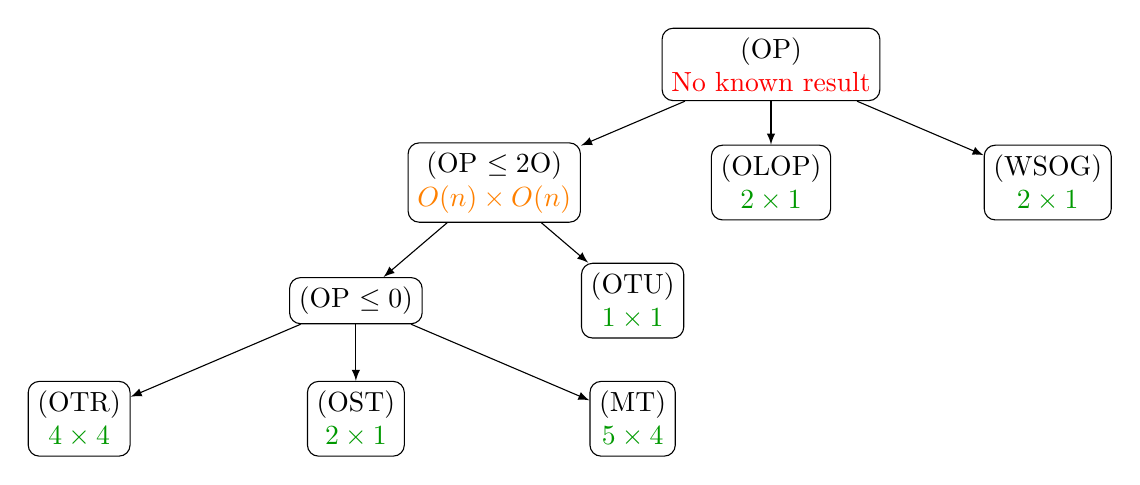
\begin{tikzpicture}[sibling distance=10em,
          edge from parent/.style = {draw,-latex},
          every node/.style = {shape=rectangle, rounded corners,
          draw, align=center}
          ]
          \node {(OP) \\ \expcolor No known result}
            child { node { (OP $\leq 2$O) \\ \lincolor $O(n) \times O(n)$}
                child { node {(OP $\leq 0$)}
                  child { node {(OTR) \\ \constcolor $4 \times 4$}}
                  child { node {(OST) \\ \constcolor $2 \times 1$}}
                  child { node {(MT) \\ \constcolor $5 \times 4$}}}
                child { node{(OTU) \\ \constcolor $1 \times 1$}}}
           child { node {(OLOP) \\ \constcolor $2 \times 1$}}
           child { node {(WSOG) \\ \constcolor $2 \times 1$}};
         \end{tikzpicture}}
      \end{center}
  \caption{A tree of inclusions between the relevant classes is shown, where an edge $(b) \rightarrow (c)$ means that $(b) \supset (c)$. 
    The classes have full names and citations given in Figure \ref{Results list figure}.}\label{Results tree figure}
\end{figure}

In Section \ref{Nonlinear section} we focus on algorithms developed for above-linear refinement on genus 0 orthogonal polyhedra.
We begin in Subsection \ref{Nonlinear definitions subsection} by defining terminology which will be used throughout the rest of the survey.
Then, in Subsection \ref{Nonlinear epsilon subsection} we sketch the epsilon unfolding algorithm of \cite{Damian_Flatland_Orourke}.
Following this, in Subsection \ref{Nonlinear delta subsection} we sketch the delta unfolding algorithm of \cite{Damian_Demaine_Flatland}. 

Following this, in Section \ref{Linear section} we focus on algorithms for grid unfolding orthogonal polyhedra with linear refinement.
In Subsection \ref{Linear zero subsection}, we sketch the algorithm of \cite{Chang_Yen} for genus zero orthogonal polyhedra.
Then, in Subsection \ref{Linear nonzero subsection}, we sketch the extension in \cite{Damian_Demaine} of the previous algorithm to genus $g \leq 2$.

Last, in Section \ref{Constant section} we sketch several algorithms for grid unfolding particular classes of orthogonal polyhedra with constant refinement.
Subsection \ref{Constant one layer subsection} focuses on unfolding one-layer polyhedra.
Then, Subsection \ref{Constant orthograph subsection} focuses on unfolding orthostacks and orthographs, including orthotubes, well-separated orthographs, and orthotrees.
Last, Subsection \ref{Constant manhattan subsection} focuses on unfolding Manhattan towers.

\section{Worse than linear refinement: epsilon and delta unfolding} \label{Nonlinear section}
The first known algorithm to establish general unfoldings of genus 0 orthogonal polyhedra, called the \emph{epsilon unfolding algorithm}, was proposed in \cite{Damian_Flatland_Orourke}.
Further results on general low-genus orthogonal polyhedra tend to follow a similar strategy, so we first introduce a meta-strategy generalizing this.

\begin{figure}
  \begin{center}
    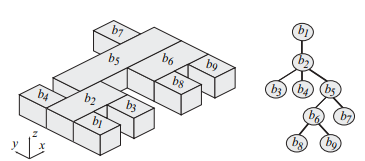
\includegraphics[width=.7\textwidth]{./figs/Unfolding_tree.png}
  \end{center}
  \caption{
    An example of an unfolding tree rooted at band $b_1$, due to \cite[Fig. 2]{Damian_Flatland_Orourke}.
  }\label{Unfolding tree figure}
\end{figure}

\subsection{Bands, unfolding trees, and spiral paths}\label{Nonlinear definitions subsection}
\paragraph{Definitions}
Fix an orthogonal polyhedron $P$.
Let $Y_0,Y_1,\dots$ be the planes which contain a vertex of $P$ and are perpendicular to the $y$ axis, sorted by increasing $y$ coordinate.
These planes can be used to slice (the solid polyhedron) $P$ into \emph{layers}, and the connected components of a layer are called \emph{slabs}.
The faces of a slab not perpendicular to the $y$ axis occur in four-face cylinders which we call \emph{bands}.
Each band has two square boundary components, called \emph{rims}.
We say that a rim \emph{encloses a face} if it bounds a (necessarily simply connected) $y$-perpendicular face.

We refer to a thin vertical rectangular strip on a $y$-perpendicular face connecting two rims as a \emph{$z$-beam}, where such a beam is allowed to have zero length corresponding with connected sides.
These form edges of a graph whose nodes are the bands of $P$, which can further be seen to be connected always and acyclic in the case that $P$ has genus $g = 0$.
In the case that $P$ has genus $g = 0$, there exists a band with a rim enclosing a face as in \cite{Damian_Demaine}, and we arbitrarily designate one such band as a \emph{root node};
there is a unique directed tree whose underlying graph is the $z$-beam graph with root node given by our choice, which we call an \emph{unfolding tree} for $P$.
See Figure \ref{Unfolding tree figure} for an example.


Let $b$ be a non-root band.
Then, we designate the rim of $b$ which is connected via $z$-beam to $b$'s parent as the \emph{front rim}, and the other as the \emph{back rim}.
In the case of the root node, we designate a rim enclosing a face as the front rim and the other as the back rim.
In either case, we designate a child of a band to be a \emph{front child} if it is connected via $z$-beam to the front rim, and a \emph{back child} if connected to the back rim.

\paragraph{The meta-strategy}
The strategy of \cite{Damian_Flatland_Orourke,Damian_Demaine,Damian_Demaine_Flatland,Chang_Yen} can be summarized as finding a \emph{spiral path} along $P$, which is a noncrossing path beginning and ending on the front rim of the root node, which spirals around each band at least once and traverses each $y$-perpendicular face at least once.
This path, thickened appropriately, will yield a cover of $P$ by a ``staircase,'' which will provide the unfolding.
The details of this unfolding can be found in \cite{Damian_Flatland_Orourke}, but we will focus primarily on the construction of the spiral path.

\begin{figure}
  \begin{center}
    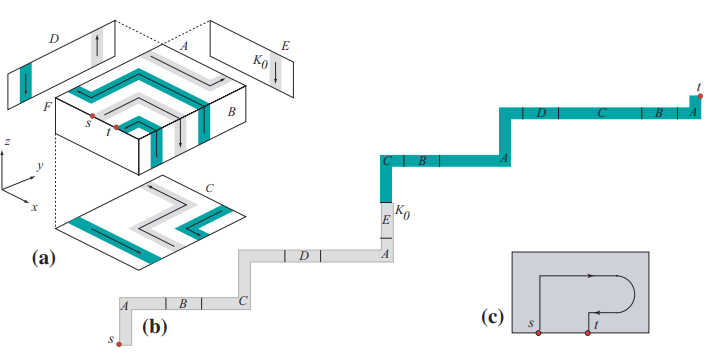
\includegraphics[width=\textwidth]{./figs/New_diagram_who_dis.png}
  \end{center}
  \caption{
    An example of a spiral path and its unfolding, due to \cite[Fig. 3]{Damian_Flatland_Orourke}.
  }\label{Box spiral figure}
\end{figure}

An example of such a spiral path as well as the accompanying unfolding is given in Figure \ref{Box spiral figure};
this is used as a base case in inductive constructions in all of \cite{Damian_Flatland_Orourke,Damian_Demaine,Damian_Demaine_Flatland,Chang_Yen}.
As is standard in the literature, we will give diagrams primarily in the style of two-dimensional figure seen in Figure \ref{Box spiral figure} (c), and expect that the reader can extrapolate the spiral paths from them. 



\subsection{The epsilon unfolding algorithm}\label{Nonlinear epsilon subsection}
\paragraph{The algorithm}
The epsilon and delta unfolding algorithms both recursively construct a spiral path for the subtree spanned by a band $b$ which ``visits'' each child (where it traverses the spiral path for each child) until it visits the last child, then ``doubles back'' and visits every other child a second time, returning to the starting point.
They share a collection of base cases analogous to that given by Figure \ref{Box spiral figure}.
The collection of such base cases is given by Figure \ref{Box spiral figure} up to symmetry; one may apply symmetries along or across the $y$ axis and ``switch'' the direction of the spiral path to give all of the base cases. 
These are distinguished in \cite{Damian_Flatland_Orourke,Damian_Demaine,Damian_Demaine_Flatland,Chang_Yen}, but we avoid doing so very explicitly for pedagogical clarity;
instead, we often exemplify the given structure for one choice of relative positions of the beginning- and end-point of the spiral path, the preferred ``direction'' of the spiral, etc., and expect that the reader can use symmetry to apply the algorithm in a broader case.\cite{Damian_Flatland_Orourke,Damian_Demaine,Damian_Demaine_Flatland,Chang_Yen}

For the epsilon unfolding algorithm, a convenient path is chosen at the inductive step.
The data mentioned above determines an initial \emph{direction} (clockwise or counterclockwise) for the spiral path to traverse, which it does until it encounters a $z$-beam from a front child.
Then, it inductively follows the spiral path for that child, exits, switches direction, and continues in the opposite direction, with $y$ coordinate farther from the front rim than the initial spiral to avoid crossing.
It continues in this process, traversing each child as possible, until it exhausts the front children.

Following this, it spirals around the band if necessary, and arbitrarily chooses a first front child to visit.
It visits this child, and the direction it travels after leaving that child is determined by the fact that the path should not be self-crossing.
Then, it follows a ``reverse process'' to that of the front children, where it continually visits the ``last'' back child until it has visited all of them.
After exiting the final back child, it ``doubles back'' in reverse direction over the entire spiral path until it reaches the front node again.
This is exemplified in Figure \ref{Epsilon figure}.

\begin{figure}
  \begin{center}
    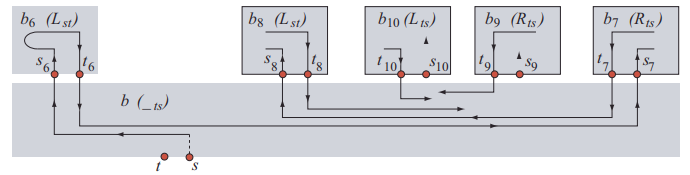
\includegraphics[width=\textwidth]{./figs/Recursive_step_example_front.png}\\
    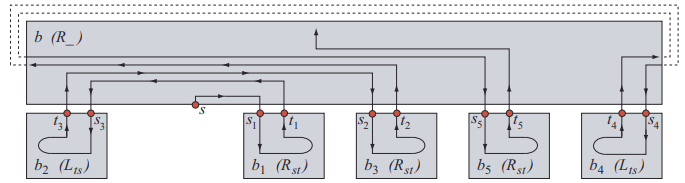
\includegraphics[width=\textwidth]{./figs/Recursive_step_example_back.png}
  \end{center}
  \caption{
    An example of a spiral path and its unfolding, due to \cite[Fig. 3]{Damian_Flatland_Orourke}.
  }\label{Epsilon figure}
\end{figure}
\paragraph{Asymptotics}
To analyze asymptotic refinement, we introduce a bit of terminology:
given a spiral path $\xi$, the \emph{path density} of $\xi$ is the maximum number of parallel paths of $\xi$ in a band of $P$.
We will use the notation $\xi_b$ for the spiral path inductively constructed to begin at the front rim of band $b$, and we will use the non-standard notation $D(\xi)$ for the path density of $\xi$.
If $D(\xi) = k$, then we have at most $k \times k$ refinement.


If $b_1,\dots,b_m$ are the children of band $b$ such that $b_i$ is visited $v_i$ times and $b_i$ is visited before $b_{i+1}$, then
\begin{equation}\label{Epsilon delta recursion equation}
  D(\xi_b) = O(m) + \max_{1 \leq i \leq m} v_i \cdot D(\xi_{b_i}).
\end{equation}
In particular, for the epsilon unfolding algorithm, all children are visited twice except for $b_m$, which is visited once, so we have
\[
  D(\xi) = O(m) + D(\xi_{b_m}) + 2\max_{1 \leq i < m} D(\xi_{b_i})
\]  
In general, this leads to a path density of $2^{O(n)}$, leading to a refinement of $2^{O(n)} \times 2^{O(n)}$, since the unfolding tree has $O(n)$ height;
in fact, Figure \ref{Exponential refinement figure} gives a family of examples which achieves $2^{\lfloor n/2 \rfloor} \times 2^{\lfloor n/2 \rfloor}$ refinement.
\begin{figure}
  \begin{center}
    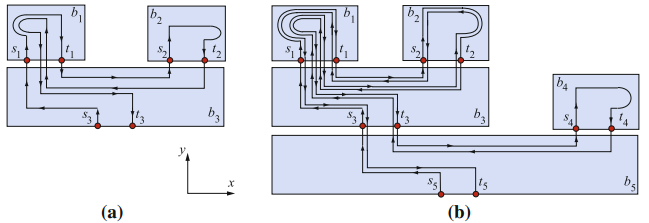
\includegraphics[width=\textwidth]{./figs/Exponential_path_density.png} 
  \end{center}
  \caption{
    The first 2 elements of a sequence of orthogonal polyhedra which are given exponential refinement by the epsilon unfolding strategy. \cite[Fig. 7]{Damian_Flatland_Orourke}.
  }\label{Exponential refinement figure}
\end{figure}

\subsection{The delta unfolding algorithm}\label{Nonlinear delta subsection}
Note that the convenient traversal of children of a band used in epsilon unfolding led to some pathological examples, where a tree of depth $O(n)$ could contain a path of length $O(n)$ such that, at each step, the edge corresponds with a traversal of a child other than the last one, and hence the path density doubled at each step.
One can remove pathologies if they are able to ensure that the ``heavy'' child is usually visited last.

To this end, let $n(b)$ be the number of nodes in the subtree spanned by a band $b$ of $P$, and designate a non-root node $b$ with parent $b'$ to be \emph{heavy} if $2n(b) > n(b')$.
Note that each node has at most one heavy child.

\paragraph{The algorithm}
First introduced in \cite{Damian_Demaine_Flatland}, the \emph{delta unfolding algorithm} is so-named because it comes as a simple improvement to the epsilon unfolding algorithm which improves refinement (hence leading the unfolding to be ``wider'') to $O(n^2) \times O(n^2)$.
To do so, delta unfolding simply ensures that it inductively visits heavy children last.
In the case of no heavy children, we follow the epsilon unfolding algorithm.

In the case of a heavy back child, this is an easy modification of the epsilon unfolding algorithm;
the first back child to visit is chosen arbitrarily, and the mapping from the first to last child visited is a permutation of the back children.
Hence we may simply perform a partial spiral such that the last back child visited (and hence the last child visited at all) is heavy.

\begin{figure}
  \begin{center}
    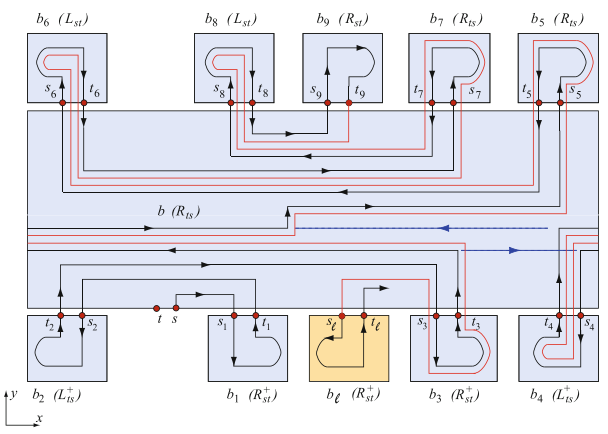
\includegraphics[width=.8\textwidth]{./figs/delta_unfolding_front.png}\\
  \end{center}
  \caption{
    An example of the delta unfolding spiral path in the case of heavy children, illustrated until traversal of the heavy child, which is highlighted in yellow.
    The figure is due to \cite[Fig. 9]{Damian_Demaine_Flatland}.
  }\label{Delta figure}
\end{figure}

In the case of a heavy front child, the argument is a bit more difficult.
In this case, we begin by ``ignoring'' the heavy front child, and performing the epsilon unfolding inductive traversal of all front and back children, then ``double back'' over the back children.
Then, noting that the ``backtrack'' is consistently able to visit the rim without crossing, it backtracks until it is possible to traverse the heavy child, at which time it does.
Then, it ``backtracks'' through the entire path as given.
See Figure \ref{Delta figure} for an illustration of this.

\paragraph{Asymptotics}
Note that a child may in general be visited at most 4 times, and heavy children are visited exactly once.
Let $R(n(b))$ be the asymptotic bound on the path density of trees with $n(b)$ many nodes.
Then, note that
\begin{align*}
   R(n(b))  
   &= \max \left\{ O(n(b)), 4 \max_{i \text{ non-heavy}} R(n(b_i)), R(n(b_{\text{heavy}}))\right\}\\
   &\leq \max \left\{ O(n(b)),4 R\left( \frac{n(b)}{2} \right), R(n(b) - 1)\right\}    .
\end{align*}
Inductively, this yields a bound of $R(n(b)) = O(n(b)^2)$;
hence our algorithm yields $O(n^2) \times O(n^2)$ refinement.
This can be shown to be sharp given a family of orthogonal polyhedra whose unfolding trees are full binary trees.

\section{Linear refinement}\label{Linear section}
\subsection{Genus 0 case} \label{Linear zero subsection}
Further improvements which modify delta unfolding appear unlikely.
It seems necessary to visit some nodes 4 times to avoid heavy children, which leads to the above asymptotics.
Instead, in \cite{Chang_Yen}, a modification of the epsilon unfolding algorithm was proposed, which substantively altered the way in which spiral paths were constructed;
letting $l(b)$ be the number of leaf nodes in the subgraph spanned by band $b$, we inductively construct a collection of $l(b)$ mutually non-intersecting spiral paths whose endpoints are adjacent on the front rim of $b$, who spiral around each band under $b$, and who unfold each leaf node under $b$ correctively.
Then, when we reach the root node, we employ a special gadget to ``stitch together'' the spiral paths into a single path suitable to unfold the polyhedron.

In addition to achieving linear refinement, this algorithm avoids the ``back and forth'' inductive routing of the delta and epsilon unfolding algorithms, leading to an arguably simpler algorithm.
As in \cite{Damian_Demaine}, we begin by making the simplifying assumptions that the root node has degree one and all internal nodes have back children;
these can be implemented with at most a constant factor ``penalty'' in refinement, by ``cutting'' offending bands.

\begin{figure}
  \begin{center}
    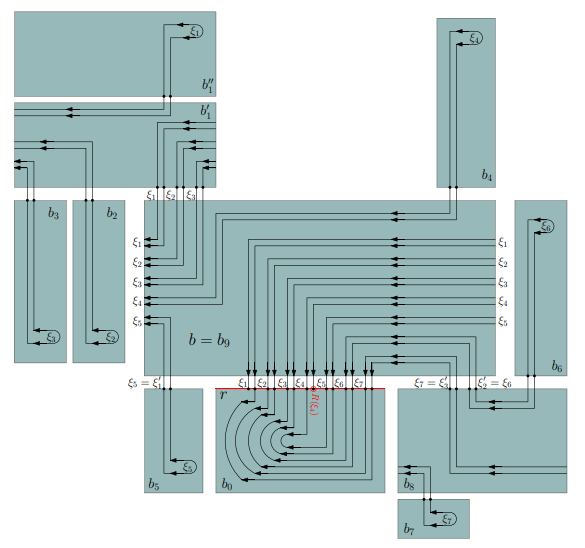
\includegraphics[width=.6\textwidth]{./figs/Linear_unfolding.png}
  \end{center}
  \caption{
    An example of the linear unfolding algorithn.
    This figure is due to \cite[Fig. 4]{Damian_Demaine}.}\label{Linear unfolding figure}
\end{figure}

Suppose for simplicity that the direction of the band $b$ is clockwise.
These directions induce a cyclic ordering of the spiral paths in each band, and the linear unfolding algorithm yields spiral paths whose order agrees with a lexicographic order on the back children, distinguishing more coarsely between children and more finely within children.
The same ordering is true of extensions of back children, which occur after the front children.
This is illustrated in Figure \ref{Linear unfolding figure}

The root node unfolding is also illustrated in Figure \ref{Linear unfolding figure}, and it is analogous to the leaf node unfoldings illustrated in Figure \ref{Box spiral figure}.
Since the inductive step ``adds'' paths rather than ``multiplying'' paths by doubling over, it can be seen that this strategy yields $O(l(b)) \leq O(n)$ path density, and hence $O(n) \times O(n)$ refinement..
This can be shown to be sharp using a family of orthogonal polyhedra whose unfolding tree is a star.

\subsection{Genus $g \leq 2$ generalization}\label{Linear nonzero subsection}
In \cite{Damian_Demaine}, the linear unfolding algorithm was extended to orthogonal polyhedra of genus $g \leq 2$.
This comes with some major impediments:
\begin{enumerate}
  \item In the genus 0 case, the graph we used to define the unfolding tree was \emph{acyclic};
    in the higher genus case, this may not be true.
  \item In the genus 0 case, there was a choice of a band with a rim enclosing a face of $P$ which served as a root node;
    such a band may not exist in the higher genus case.
  \item In the genus 0 case, the back rim of each leaf node enclosed a face of $P$.
    this may not be true in the higher genus case.
\end{enumerate}
For an example where all of these fail, see the genus 3 polyhedron in Figure \ref{Orthogonal polyhedron figure}.

In order to establish results in higher genus, new graphs are constructed in \cite{Damian_Demaine} to replace the unfolding tree;
form the \emph{rim graph} $G_r$ by replacing each node in the graph underlying the unfolding tree with two connected nodes (one for each rim), and replacing each edge with edge between the corresponding rims.
Edges in this graph are either \emph{$b$-edges} or \emph{$z$-edges} depending on whether they come from a band or a $z$-beam.
Rims are called \emph{face nodes} if they enclose a face, and \emph{nonface nodes} otherwise.

The following lemma is due to \cite[Lem. 3.1.1]{Damian_Demaine}:
\begin{lemma}
  If the polyhedron $P$ has genus $g \leq 2$, then there is a direction for slicing $P$ such that $G_r$ includes a face node $r_F$.
\end{lemma}
This is proved by assuming for WLOG that none of the ``extreme faces'' (marked by extreme $y$-value) are simply connected in any of the six directions, and categorizing inner bands in such faces as \emph{caves} or \emph{holes}.
If a cave band ``contributes nothing to the genus,'' then it induces a rim enclosing a face;
a counting argument on the genus implies that one such band must exist.

This fixes our second issue.
We can begin solving our third issue by the following Lemma, due to \cite[Lem. 3.1.2]{Damian_Demaine}:
\begin{lemma}
  $G_r$ is connected and contains no nonface leaf nodes.
\end{lemma}
Connectivity follows from connectivity of $P$, and no nonface leaf nodes may exist, since a leaf node may not be connected via $z$-beam to another node by degree;
this requires that the non-band surface it's connected to be simply connected, so every leaf node encloses a face.

With these established, edges in simple cycles are removed arbitrarily to construct a \emph{rim spanning tree}  $T_r$ of $G_r$.
The following theorem, due to \cite[Thm. 3.1.1]{Damian_Demaine}, almost simultaneously fixes all of our impediments in the higher genus case.
\begin{theorem}
  The number of nonface leaf nodes in $T_r$ is at most the genus $g$ of $P$.
\end{theorem}
Then, we construct an unfolding tree $T$ with vertices given by the bands, by simply contracting the $b$-edges of $T_r$.
Our construction, which ensures that no nonleaf nodes have only front children, ensures that the contraction yields a bijection between the leaves of $T$ and the leaves of $T_r$.
Hence our tree $T$ has at most $g$ nonface leaf nodes.

In the case that there are no nonface leaf nodes, the linear unfolding algorithm works as described above, using unfolding tree $T$.
Otherwise, we break into cases depending on whether there are one or two nonface leaf nodes.

\begin{figure}
  \begin{center}
    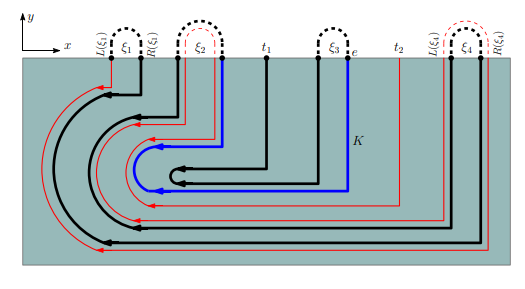
\includegraphics[width=.6\textwidth]{./figs/Nonface_leaf.png}
  \end{center}
  \caption{
    An example of the stitching-together of spiral paths at the root band in the case of two nonface leaf nodes.
    The points $L(\xi_i)$ and $R(\xi_i)$ refer to the endpoints of spiral path $\xi_i$, and $t_i$ is the endpoint of the spiral path of the $i$th nonface leaf node.
    This figure is due to \cite[Fig. 11.]{Damian_Demaine}.}\label{Nonface leaf figure}
\end{figure}

In the case of one nonface leaf node, we employ a gadget at the root which connects the (ordinary) spiral paths to and from leaf nodes together, ending on a spiral path which travels to the back rim of the leaf node, where it stops.
In the case of two nonface leaf nodes, the gadget used at the root connects paths such that the full spiral path begins and ends at the back rims of the two nonleaf nodes.
See Figure \ref{Nonface leaf figure} for an example.
We refer the reader to \cite{Damian_Demaine} for details.

There are challenges extending this algorithm to a more general genus;
in general, we may not have a root node enclosing a face to choose to begin at.
Further, $T_r$ may have at least 3 nonface leaf nodes, so we will not be able to ensure that each nonface leaf node has an endpoint of the spiral path.

\begin{figure}
  \begin{center}
    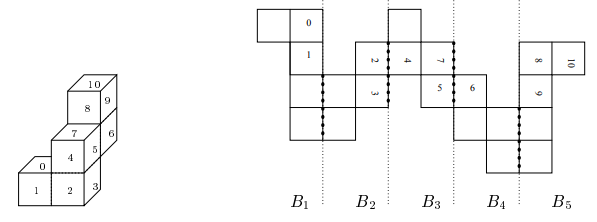
\includegraphics[width=.8\textwidth]{./figs/Orthotube_unfolding.png}\\
  \end{center}
  \caption{
    An example of an unfolding of an orthotube.
    The figure is due to \cite[Fig. 10]{Biedl_Demaine}.
  }\label{Orthotube figure}
\end{figure}
\section{Constant refinement miracles}\label{Constant section}
Outside the general genus $g \leq 2$ case, there are algorithms known to unfold several classes of orthogonal polyhedra with refinement invariant to the data of the polyhedron.
These are listed in the lower portion of Figure \ref{Results list figure}.
In this section, we will give definitions of some such classes, as well as sketches of their unfolding algorithms.

\subsection{One-layer polyhedra}\label{Constant one layer subsection}
We say than a \emph{one-layer polyhedra} is a polyhedra with one layer, i.e. one where the $y$-values of all vertices are one of two distinguished values $y_0,y_1$.
In \cite{Liou}, edge unfoldings are constructed for several classes of one-layer polyhedra, including many cases of arbitrary genus.
Following this, \cite{Chang_Yen} noted techniques from the linear unfolding algorithm (with unfolding tree given as a spanning tree of the graph of $z$-beams) can be used to unfold arbitrary one-layer polyhedra with only $2 \times 1$ refinement applied to $2(g-1)$ faces (without refinement on all other faces);
these are two refinements per edge other than the edge between the root and its child, yielding $2(g - 1)$ refinement corresponding with the $g$ edges in the unfolding tree.
We refer the reader to \cite{Chang_Yen} for details.

\subsection{Orthographs and orthostacks} \label{Constant orthograph subsection}
Some of the first classes of orthogonal polyhedra considered for unfolding are \emph{orthotubes} and \emph{orthostacks}, which both appear somewhat like ``generalized cylinders;'' they appear to follow a simple curve, with simple cross sections along the curve.

More specifically, an orthogonal polyhedron is called an \emph{orthostack} if it has simply connected layers. 
It is called an \emph{orthograph} if it is made by gluing rectangular ``bricks'' together along their faces, and it is called an \emph{orthotube} if it is an orthograph which forms either a chain or a cycle, such that two non-adjacent bricks intersect in $\leq 1$-dimensional faces of the intersection of each brick with one of its neighbors.
It is called an \emph{orthotree} if its graph instead forms a tree.

We refer to a box in an orthograph as a \emph{junction} if it is not a tube block.
Say that an orthograph is \emph{well-separated} if it does not contain adjacent junctions.

\paragraph{Orthostacks}
We sketch the argument given in \cite{Biedl_Demaine}, noting that our convention ``rotates'' the orthostack such that it has simply connected layers with respect to $y$-planes, whereas theirs cuts along $x$-planes.
Since each layer is simply connected, it consists of exactly one band.
We cut each band in order to make a strip, and we spread the strips out in order of increasing $y$-coordinate;
between each strip we attack $y$-faces in a connected and overlap-free manor.

For the $i$th layer, define the \emph{left $i$th band} $L_i$ to be the lower half of the $i$th band, and define the \emph{right $i$th band} $R_i$ to be the upper half of the $i$-th band.
Define $D_i$ to be the union of the $y$-faces with $y$-coordinate $Y_i$.
By Convention we define $R_0 = L_{k+1} = \emptyset$.

It suffices to unfold each union of adjacent ``half-layers'' $R_i \cup D_i \cup L_{i+1}$ and connect each of these components without overlap.
The unfolding of each $R_i \cup D_i \cup L_{i+1}$ is done by cutting $D_i$ into pieces, cutting each of $R_i$ and $L_i$ once into strips, and attaching all of these together in an appropriate manner.
We refer the reader to \cite{Biedl_Demaine} for additional details and for the argument on connecting these pieces.
The cuts on $D_i$ as well as the separation of half-layers is necessary, as Figure \ref{Orthogonal polyhedron figure} included an example of an orthogonal polyhedron without an edge unfolding.

\paragraph{Orthotubes}
Choose an ordering $B_0,\dots,B_{k-1}$ for the blocks comprising an orthotube $P$ such that $B_i,B_{i+1}$ are adjacent.
We refer to the \emph{surface of a block} as its faces within the orthotube, and we iterate through $B_i$ with increasing $i$, giving an unrefined unfolding of the surface of each block as we go.

\begin{figure}
  \begin{center}
    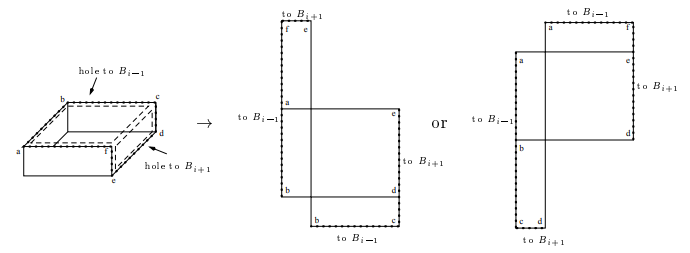
\includegraphics[width=.8\textwidth]{./figs/Corner_unfolding.png}\\
  \end{center}
  \caption{
    The two unfoldings considered for corner blocks.
    The figure is due to \cite[Fig. 11]{Biedl_Demaine}.
  }\label{Corner unfolding figure}
\end{figure}

To do so, we give separate unfoldings of a ``tube block'' with holes on opposite sides and a ``corner block'' without that.
Tube blocks are unfolded by cutting along one of the four edges which are not on the boundary of a hole (with choice dependent on the previous block), and corner blocks are unfolded with one of the two unfoldings outlned in Figure \ref{Corner unfolding figure}.
These are stitched together in such a way that traversing the orthotube will yield a corresponding rightward-traversal of the unfolding.
We refer the reader to \cite{Biedl_Demaine} for more details.
 
\paragraph{Other classes of orthographs}
An algorithm for grid-unfolding well-separated orthotrees without refinement was proposed in \cite{Damian_Flatland_Well_Separated} using an analogous argument to the case of orthotubes, this time breaking into cases based on the degree of the node. 
Without the well-separated assumption, an algorithm was proposed in \cite{Damian_Flatland_Better} to grid-unfold orthotrees with $4 \times 4$ refinement, recursively on the height of the tree;
this algorithm is significantly more complicated than that of \cite{Damian_Flatland_Well_Separated}, since the adjacent junctions in a non-well-separated orthotree may ``get in the way of each other.''

In \cite{Ho_Chang_Yen}, the results of \cite{Damian_Flatland_Well_Separated} are extended to a grid unfolding of well-separated orthographs using $2 \times 1$ refinement;
this is one of very few results generating unfoldings of polyhedra of arbitrary genus, along with results from \cite{Chang_Yen} on one-layer polyhedra.
This time, care is given to modifying the dual graph of a well-separated orthograph to replace the ``star'' local to each junction with a cycle, and to distinguish those edges from non-junction edges.
An \emph{unfolding path} in the dual graph is constructed with passes through all edges of the modified dual graph, which doesn't pass through two junction edges simultaneously or ``double back'' over non-leaf nodes.
The unfolding takes place along the unfolding path, employing similar casework to \cite{Damian_Flatland_Well_Separated}.
We refer the reader to \cite{Ho_Chang_Yen} for details.



\subsection{Manhattan towers}\label{Constant manhattan subsection}
For orthostacks, cross sections were allowed to have, with increasing $y$, ``expanding'' or ``contracting'' layers, so long as each layer was simply connected.
We may instead require that the base layer is simply connected and that each layer is contained in every layer of lower $y$ coordinate;
such polyhedra are called \emph{Manhattan towers}.

\begin{figure}
  \begin{center}
    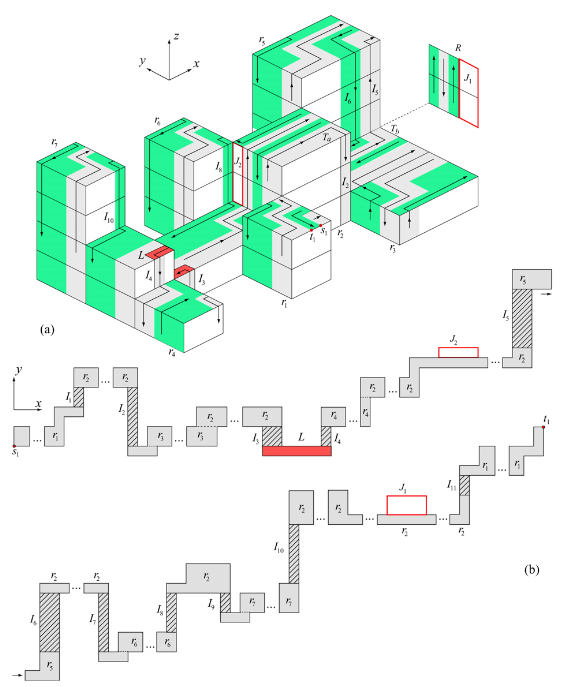
\includegraphics[width=.8\textwidth]{./figs/Manhattan_tower_unfolding.png}\\
  \end{center}
  \caption{
    An unfolding of a Manhattan tower, due to \cite[Fig. 12]{Damian_Flatland_Orourke_Manhattan}.
  }\label{Manhattan tower unfolding figure}
\end{figure}

These can be reoriented such that the layers run perpendicular to the $z$ axis; then, taking ``slices'' perpendicular to the $y$ axis and taking connected components of each slice, a Manhattan tower can be decomposed into a collection of simply connected \emph{slabs}.
The unfolding algorithm for Manhattan towers unfolds each slab analogously to the epsilon unfolding algorithm, and ``sutures'' the unfoldings of the slabs together.
For an example of this unfolding, see Figure \ref{Manhattan tower unfolding figure}.
We refer the reader to \cite{Damian_Flatland_Orourke_Manhattan} for more details.

\printbibliography
\end{document}
